\section{Bivalent Binding Process}

%In section \ref{sec:rebinding}, we explained the rebinding effect in a receptor-ligand system consisting of receptors and ligands that move freely, i.e. without being connected to each other.
%Such systems, respectively its molecules, are called \textit{monovalent}.

%arbitrary/artificial. highlight/visualize
After having analyzed a purely theoretical example in order to visualize the quality of the estimation for the rebinding effect,
%compare the minimal rebinding effect to the real rebinding effect.
%some important properties/relations of the rebinding effect,
we continue to examine a \textbf{binding process}, being the original motivation for the investigations of the rebinding effect.
%analyzing/examining/investigating/describing

\subsubsection*{Multivalent System}

In section \ref{sec:rebinding}, we introduced the rebinding effect as a memory effect included in a system of receptors and ligands, without any connection of the ligands.
However, one can distinguish between \textbf{monovalent} and \textbf{multivalent} binding processes. % (see ...).
Whenever the receptor molecules are spatially preorganized, the corresponding binding process is denoted as multivalent.
We can imagine that as several receptors being connected by a linker. %\marginpar{image}

%\begin{figure}[!ht]
%	\label{fig:bivalent}
%	\centering
%	\includegraphics[width=0.25\textwidth]{figures/bivalent2}
%	\caption{Bivalent System.}
%\end{figure}
%Accordingly, given a structure of multivalent receptors, it sounds plausible to design fitting ligands, i.e. ligands of the same valency.  %multivalent
%\\

%bind to monovalent or multivalent receptors?
Especially the bivalent or polyvalent case often is observed in nature. \marginpar{?}
These systems are of significant interest for pharmaceutical and technical applications. If the ligands are linked to each other in an appropriate way to match the preorganized receptor molecules and, thus, are also presented multivalently, then extremely high binding affinities are often observed, which is conjectured to originate by the rebinding effect. %be caused
\begin{figure}[!ht]
	\centering
	\includegraphics[width=0.25\textwidth]{figures/trivalent_binding.jpg}
	\caption{Trivalent System.}
	\label{fig:trivalent}
\end{figure}
%For the monovalent case, the mathematical modeling of its kinetics is well understood. monovalent = reversible? or why not of interest??? -> trivial min. reb. eff
This is clarified in figure \ref{fig:trivalent}, representing a trivalent system. If one of the connected ligands dissociated from its receptor, after being in the completely bound state (triple bound), then the probability of the ligand to be still close to its receptor and to rebind, is high.
We can imagine that this rebinding effect is even higher than it would have been the case in a monovalent system, since the ligand is kept at its place by its two connected ligands.
%after that the trivalent ligand was completely bound to the trivalent receptor, 

The strength of this ``adherence'' depends also from the flexibility of the linker. They can be either rigid/stiff or more flexible. A rigid linker holds the connected ligand more strongly at its place than a flexible linker. This relation is shown by Weber et al\cite{weber2012}. 
\\

The mathematical modelling of a monovalent system is well understood. Furthermore, if defined on the two macro states ``unbound'' and ``bound'', the computation of the minimal rebinding effect in such a system yields only the trivial solution, by theorem \ref{thm:reversible_trivial}.

Hence, as the the easiest multivalent case, we consider a \textbf{bivalent} process.
Such a system can be described by three macro states: ``unbound'', ``singly bound'' and ``doubly bound'', depicted in figure \ref{fig:bivalent_states}. %modelled. shown/depicted
\begin{figure}[h] %[!ht]
	\centering
	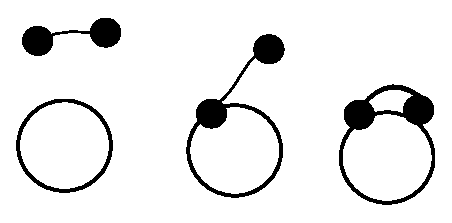
\includegraphics[width=0.4\textwidth]{figures/bivalent_states}
	\caption{Possible macro states of a bivalent system.}
	\label{fig:bivalent_states}
\end{figure}
This model can be represented by the reversible reactions
\begin{equation}
\begin{aligned}
\label{eq:reactions}
\mathrm{LL} + \mathrm{RR} & \rightleftharpoons \mathrm{L(LR)R}, \\
\mathrm{L(LR)R} & \rightleftharpoons \mathrm{(LRLR)}, \\
\mathrm{LL} + \mathrm{RR} & \rightleftharpoons \mathrm{(LRLR)},
\end{aligned}
\end{equation}
resulting in a transition rate matrix
\begin{equation*}
Q_c = 
\begin{pmatrix}
	-(k_{01} + k_{02})[RR]	& k_{01}[RR] 		 & k_{02}[RR]  \\
	k_{10}      			& -(k_{10} + k_{12}) & 	k_{12}	\\
	k_{20}					&	k_{21}			 & -(k_{20} + k_{21})
\end{pmatrix},
\end{equation*}
depending on the concentrations of the bivalent receptor molecules $[RR]$.
This matrix is constructed in the same fashion as explained in section \ref{sec:rebinding} for the monovalent case and as well describes changes of concentrations by the ordinary differential equation
\begin{equation*}
\dot{x}^T = x^T Q_c.
\end{equation*}
By this equation, changes of concentrations $x^T = ([LL], [L(LR)R], [(LRLR)])$ in this system can be observed/described.
\\

We can either measure or determine some plausible/feasible association/dissociation constants.
Remark: the last reaction equation in \eqref{eq:reactions} should have \textbf{very} small association and dissociation constants, since transitions from the unbound state directly to the bound state or vice versa are not realistic; if they happen then extremely rarely. However, we don't set them $0$, in order to avoid a sparse transition rate matrix $Q_c$.
%since we don't want to have a sparse transition rate matrix. %in order to get plausible/feasible results

\subsubsection*{Rebinding Effect}

We are in the situation that we are given a process which can be \textbf{interpreted} as a projection, while we do \textbf{not} know the original process and therefore cannot compute the actual rebinding effect.
However, we assume that by the unknown projection, there is some rebinding effect included in $Q_c$.
Assuming that it is clustered in terms of overlapping membership functions $\chi = XA$, we again solve optimization problem \eqref{eq:optimization} to derive the minimal rebinding effect as an estimation. \marginpar{Schur}
%In order to estimate it, we come back to compute the minimal rebinding effect.
\\

Need: eigenvectors/Schur vectors of $Q_c$ in order to compute the minimal rebinding effect included in this system.
It does not play a role if the original system was reversible or non-reversible, since we use Schur vectors to solve this problem.
\\

When is $Q_c$ reversible or non-reversible?
\\

%deeper/better understand
%In order to understand such a system, 
We consider it at first as an artificial system, by inserting convenient association and dissociation constants in order to obtain general informations about bivalent systems. Afterwards we examine a real system.
\subsubsection*{Artificial Binding Process}

First try: choice as in Weber and Fackeldey\cite{weber2014}.
\begin{itemize}
	\item For the reaction ``unbound'' $\leftrightarrow$ ``singly bound'': very high association $k_{01}$, low dissociation $k_{10}$
	\item For the reaction ``singly bound'' $\leftrightarrow$ ``doubly bound'': high association $k_{12}$, very low dissociation $k_{21}$
	\item For the reaction ``unbound'' $\leftrightarrow$ ``doubly bound'': very low association $k_{02}$, very low dissociation $k_{20}$
\end{itemize}

These parameters describe a system with desirable properties, since we want to obtain a high occupation of the receptors. %want to obtain/reach/achieve a high occupation
%It is a system where 
Unbound ligands have a strong preference to the single bound state, while dissociations do not happen often.
From the singly bound state to the doubly bound state happens still quite often, while dissociating not.
Going directly from unbound to doubly bound and vice versa can almost be neglected.

\begin{figure}[!ht]
	\label{fig:concentration_rebinding}
	\centering
	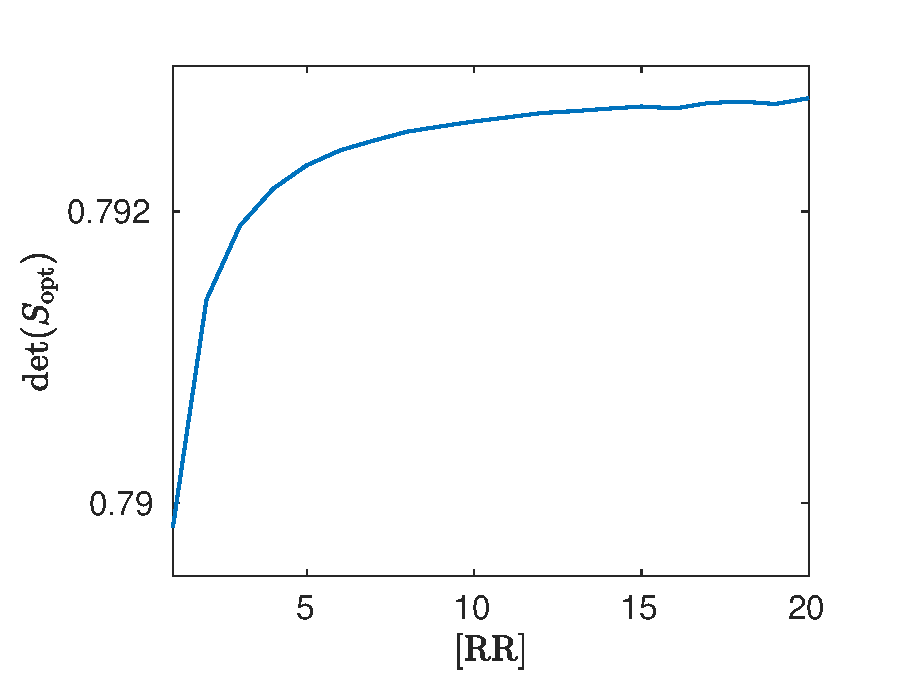
\includegraphics[width=0.55\textwidth]{figures/bivalent/concentration_rebinding}
	\caption{The minimal rebinding effect of $Q_c$ depending on the concentration $\mathrm{[RR]}$ of receptor molecules.}
\end{figure}

%Even though the difference of $\det(\Sopt)$ is not very large, we can clearly see a tendency of ..

In figure \ref{fig:concentration_rebinding}, we see that with increasing concentration of receptor molecules, the minimal rebinding effect decreases.
Even though the resulting difference of $\det(\Sopt)$ is not very large, this tendency is unambiguous. \marginpar{included in model?}
That makes sense: in a system with a large concentration of receptors, a ligand dissociating from a receptor is more likely to be already close to another receptor. If they bind, rebinding is prevented.
%Though have to keep in back-mind that the estimation can be rather good or rather bad..
\\

Even though this result qualitatively makes sense, it \textbf{should not}.
%The model consisting of the states ``unbound'', ``singly bound'' and ``doubly bound'' cannot distinguish if a dissociated ligand binds again
The model \eqref{eq:reactions} cannot distinguish if a dissociated ligand rebinds to its receptor or if it binds to a close receptor.
\\

Accordingly to Weber and Fackeldey\cite{weber2014}, this decreasing rebinding effect represented in figure \ref{fig:concentration_rebinding} can be explained by a decrease in the transition regions between the binding events caused by the increased receptor concentration.
\\

For \textbf{low} receptor concentrations the result is plausible; bindings shortly after a dissociation are likely to be a \textbf{rebinding}, since there are no other receptors nearby.
However, in realistic models the receptor concentration is higher.
\\

%Can binding events between different receptors be distinguished in the model \eqref{eq:reactions}?

%If not..
We need better models in order to correctly include rebinding effects. How?
%in order to correctly include rebinding effects in a model
\\

The presented model does not include enough informations/states to distinguish between a rebinding and a normal binding, since a dissociated ligand possesses no memory about the previous binding.
How could that be included?
Some approaches
\begin{itemize}
	\item considering larger systems, i.e. systems with more informations/ more states than just ``bound'', ``singly bound'', ``doubly bound'', making it possible to distinguish between rebinding and other bindings
	\item switching from the molecular kinetic to the molecular dynamic point of view: informations about the rebinding effect could be detected by simulations; i.e. generate a trajectory and analyze it for rebinding events \marginpar{Bettina Keller}
\end{itemize}
Finally one further outlook would be to compute the rebinding effect for time-dependent systems as well\cite{fackeldey2017}.
Consequent enhancement of PCCA+. Recently improved to non-reversible processes. New extension: including time-dependent systems by coherent sets (metastable sets with time) \cite{weber2017coherent}.

%\subsubsection*{Real existing binding process}
\subsubsection*{Real Binding Process}

Something with low receptor-concentrations.
\\

Picture

%%Remark: chemical processes are often \textbf{non-reversible}, see Fackeldey and Weber\cite{fackeldey2017}.
\newpage